\documentclass[a4paper,12pt]{article}

\title{A Reinforcement Learning Agent for Checkers\\based on MCTS and TD($\lambda$)}
\author{Alexander Pluska}

\usepackage{amsmath,amssymb,amsthm}
\usepackage{ wasysym }
\usepackage{ stmaryrd }
\usepackage{ mathpartir }
\usepackage{bussproofs}
\usepackage{enumerate}
\usepackage{tikz-qtree}
\usepackage{stackengine}
\usepackage{wrapfig}

	
\usepackage{hyperref}% http://ctan.org/pkg/hyperref
\usepackage{cleveref}% http://ctan.org/pkg/cleveref

\theoremstyle{definition}
\newtheorem{theorem}{Theorem}[section]
\theoremstyle{definition}
\newtheorem{corollary}[theorem]{Corollary}
\theoremstyle{definition}
\newtheorem{lemma}[theorem]{Lemma}
\theoremstyle{definition}
\newtheorem{proposition}[theorem]{Proposition}
\theoremstyle{definition}
\newtheorem{definition}[theorem]{Definition}
\theoremstyle{definition}
\newtheorem{example}[theorem]{Example}

\DeclareMathOperator*{\argmax}{arg\,max}

\begin{document}
	
	\maketitle
	
	\begin{abstract}
		The goal of this project is to implement a reinforcement learning agent for checkers. The used algorithm is inspired by early versions of AlphaGo~\cite{silver2016mastering}, although heavy modifications had to be undertaken to accommodate for lack of computational resources. In particular the policy and value network are merged into one and during Monte Carlo Tree Search leaf nodes are evaluated only via value network and not via roll-out.
	\end{abstract}
	
	\section{Introduction}
	
	Having followed the development of AlphaZero in awe, I thought it would be interesting to mimic some of their ideas for my own reinforcement learning agent. However with a naive single threaded Python implementation the agent needs to spend at least .5s at each position just to get to a reasonable depth during tree search, i.e. one that at least recognizes simple wins as such. This means that each simulated game needs at least 1 minute time. To achieve convergence AlphaZero required many hundreds of thousands simulations~\cite{silver2018general}. This could be achieved though massive parallelization, incredible computing resources and certainly also a much more efficient implementation. Even though checkers of course is significantly simpler than Go his kind of learning would require many years on my machine.
	
	The first adaptation is instead of two networks, a distinct policy and a valuation network, to use only one valuation network, which would completely determine the policy function via tree search and negamax.
	
	The second adaptation is to use a much more shallow network, with just two convolutional layers, specifically adapted to checkers, followed by a fully connected layer.
	
	In early versions of AlphaGo the agent was bootstrapped by supervised learning on expert moves~\cite{silver2016mastering}. However for checkers a database of such expert moves is not readily available and creating it is beyond the scope of the project, so instead the value network is bootstrapped on random positions with material count as a target.
	
	To ensure termination the game is augmented with an additional rule: The game ends immediately in a draw when a position is repeated. Clearly if there exists a winning strategy from a position then there exists one that avoids repetitions, so an optimal policy for the augmented game is also optimal for usual checkers.
	
	Finally with only these adaptations a problem was encountered where the value network would reach an equilibrium evaluating each position as a draw. During the training positions with many kings would be reached from which the agent was unable to convert a win even with overwhelming advantage. Therefore self play is not immediately performed from the stating position but instead from random positions with reduced material, i.e. endgames.
	
		
	\begin{wrapfigure}{r}{0.5\textwidth}
		\begin{center}
			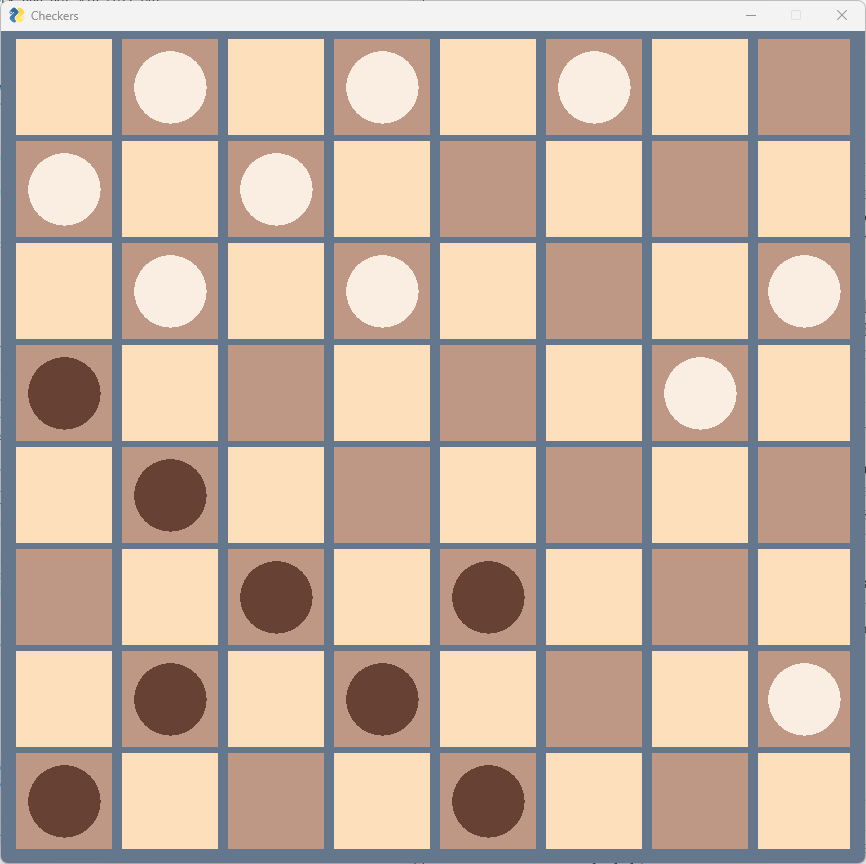
\includegraphics[width=0.48\textwidth]{gui.png}
		\end{center}
		\caption{A simple gui to observe games}
	\end{wrapfigure}

	In a funny way this is similar how chess is often first taught to children: At first the values of the different pieces are explained and the children just play to greedily maximize their material count. Then endgames are taught, in particular how to checkmate with reduced material. Finally more complex concepts are learned, of course also through other mechanisms, but also through play.

	
	Additionally I implemented a GUI that allows the user to watch games played by the agent, e.g. during self-play, and also watch games against other agents during evaluation.
	

	\section{Learning}
	
	Before explaining learning let us first discuss in depth how the policy function works. At the foundation lays a CNN with three layers that reflect the geometry of the board. As an input the CNN takes a board position encoded similarly to the encoding used in AlphaZero~\cite{silver2017mastering}, i.e. it takes a 4x32 tensor where the first row one-hot encodes the position of dark men, the second of dark kings etc. Then a first convolutional layer is applied with a 12 element kernel and stride of 4, i.e. containing the information of each three consecutive rows, extracting 8 features. The 6 layers are then combined before applying a fully connected linear layer. At each stage ReLU is used as an activation. Finally a Sigmoid function is applied to obtain an evaluation between $0$ and $1$. During learning adam is used as an optimizer.
	
	Having this net a position is evaluated via an Monte-Carlo-like tree search as follows: First create a node with the initial position and set its number of expansions to 0. Repeatedly expand this node as follows:
	\begin{itemize}
		\item If a node with $0$ expansions is to be expanded, add a child to the node for each legal move in its position and expand each of them until no more captures are possible. Then evaluate the leaves with the neural net and compute the implied evaluation of the position via negamax, i.e. 
		$$ev(\text{node}) = \max\{1 - ev(\text{child})\:|\:\text{child}\in\text{children}\}$$
		where the evaluation at each node is from the perspective of the party that has the move.
		\item If a node $n$ already has expansions, expand the child $c$ for which the value of
		$$1-ev(c) + \sqrt{2\cdot\frac{\log(\text{expansions}(n))}{\text{expansions}(c)}}$$
		is maximal, ensuring a trade-off betweeen exploration and exploitation. Finally update the value of the original node accordingly.
	\end{itemize}
	Perform expansions until some time limit is reached. Then choose the move associated with the child with minimal evaluation, i.e. minimal predicted value for the opponent.
	
	Learning is performed in three stages:
	
	First the net is initialized to approximate the material value of positions. This is done by supervised learning on 100000 randomly generated positions.
	
	In a next stage 100 Games of self-play and learning are performed from endgame positions. The learning is done on batches of 10 played games using TD(0.9), i.e. after each game a list the positions $p_0,\dots, p_n$ from the game is used as input data for the training and the targets $t_i$ are computed from the evaluations $e_i$ that were computed during the game by setting $t_n$ as the result of the game and iteratively $$t_{i-1} = 0.9t_i + 0.1e_{i-1}$$
	The learning on batches was done to avoid over-fitting, but was probably insufficient.
	
	Finally the agent learns through self-play from the original position after $2$ random moves. Again learning was done in batches of 10. The total number of games played was only 300. Due to unknown issues, perhaps related to garbage collection, the agent would sometimes hang up during evaluation, making longer training infeasible.
	
	Self-play is performed on the cpu while learning is performed on a gpu.
	
	\section{Evaluation}
	
	For evaluation agents from multiple stages of learning were pitted against each other in a round-robin tournament. There were 7 contestants
	\begin{itemize}
		\item The agent after only the supervised learning (bootstrapped)
		\item The agent after endgame training (endgame)
		\item The agents after $100$, $200$ and $300$ games (100games, 200games, 300games)
		\item A baseline agent playing random moves (random)
		\item A checkers engine (easy) programmed by Ed Gilbert~\cite{CheckerBoard}, the dll of which I accessed from python via ctypes. This is a weak engine which can be beaten even by beginners with some effort.
	\end{itemize}

	The results of the tournament can be seen below. As one can see by far the strongest version of the engine was the bootstrapped version, which just predicts material.
	\begin{center}
		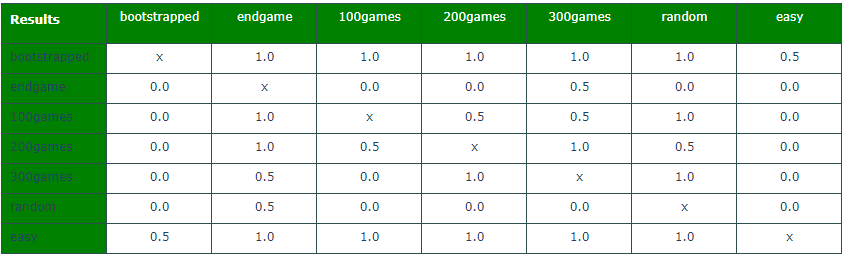
\includegraphics[width=\textwidth]{evaluation}
	\end{center}
	
	\section{Takeaway}
	
	The poor performance of the agent can be explained by different factors, however the most convincing is in my opinion that 300 games simply dont constitute enough data to train neural network with 500+ weights. While the initial agent from bootstrapping was promising, even drawing the easy engine, it had much more data to work on (100000 positions). In particular since at each stage only 10 games $\sim$ 1000 positions were considered the choice was really between miniscule learning progress or over-fitting, and what ended up happening was probably a mix of both, with a bias to the latter. While python was great for prototyping, it reinforced the bottleneck of not being able to simulate a sufficient number of games. For a future implementation I would choose a much more simple evaluation function, e.g. a single linear layer, that is less prone to over-fitting and focus on providing an optimized and possibly parallelized simulation, such that sufficient data can be generated.
	
	
	\bibliographystyle{plain}
	\bibliography{report}
	
\end{document}